% This LaTeX file contains your written lab questions.  You may answer these
% questions just by inserting your answer into this document.  You are not
% *required* to do your homework in LaTeX, but it's quite likely to be easier
% than e.g. the equation editor in OpenOffice Writer or Microsoft Word.
\documentclass{article}

\usepackage{amsmath}
\usepackage{amssymb}
\usepackage{algpseudocode}
\usepackage{algorithmicx}
\usepackage{tikz}

\usetikzlibrary{positioning}

\begin{document}

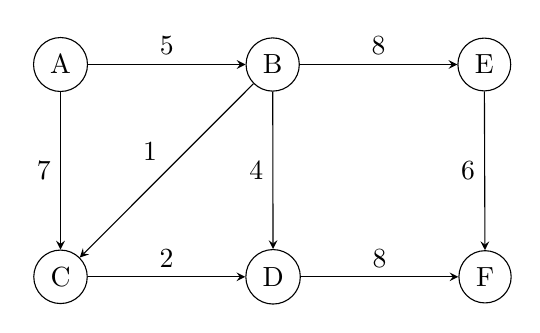
\begin{tikzpicture}[node distance=20mm and 20mm]
    \tikzstyle{vertex}=[circle,draw]
    \tikzstyle{edge}=[-stealth]
    
    \node[vertex] (A) {A};
    \node[vertex] (B) [right=of A] {B};
    \node[vertex] (C) [below=of A] {C};
    \node[vertex] (D) [right=of C] {D};
    \node[vertex] (E) [right=of B] {E};
    \node[vertex] (F) [right=of D] {F};
    
    \draw[edge] (A) to node[above] {5} (B);
    \draw[edge] (A) to node[left] {7} (C);
    \draw[edge] (B) to node[above left] {1} (C);
    \draw[edge] (B) to node[left] {4} (D);
    \draw[edge] (B) to node[above] {8} (E);
    \draw[edge] (C) to node[above] {2} (D);
    \draw[edge] (D) to node[above] {8} (F);
    \draw[edge] (E) to node[left] {6} (F);
\end{tikzpicture}

\vspace*{5mm}\par\textbf{Problem 1.} Perform a breadth-first search of the graph starting from vertex A.  Give the number of steps to reach \emph{every} other vertex.  Additionally, give the order in which the vertices are \emph{first} witnessed; that is, give the order in which they first enter the queue (and not necessarily the order in which they are explored).\par

%%%%%%%%%%%%%%%%%%%%%%%%%%%%%%%%
%% TODO: put your answer here %%
%%%%%%%%%%%%%%%%%%%%%%%%%%%%%%%%

\vspace*{10mm}\par\textbf{Problem 2.} Use Dijkstra's algorithm on this graph starting from vertex A.  Give the cost of the least-cost path to \emph{every} other vertex.  Additionally, give the order in which the vertices are \emph{first} witnessed; that is, give the order in which they first enter the equeue (and not necessarily the order in which they are explored).\par

%%%%%%%%%%%%%%%%%%%%%%%%%%%%%%%%
%% TODO: put your answer here %%
%%%%%%%%%%%%%%%%%%%%%%%%%%%%%%%%

\vspace*{10mm}\par\textbf{Problem 3.} Give two valid topological sorts of this graph.\par

\begin{center}
    \begin{tabular}{||c c c c||} 
     \hline
     Col1 & Col2 & Col2 & Col3 \\ [0.5ex] 
     \hline\hline
     1 & 6 & 87837 & 787 \\ 
     \hline
     2 & 7 & 78 & 5415 \\
     \hline
     3 & 545 & 778 & 7507 \\
     \hline
     4 & 545 & 18744 & 7560 \\
     \hline
     5 & 88 & 788 & 6344 \\ [1ex] 
     \hline
    \end{tabular}
\end{center}

%%%%%%%%%%%%%%%%%%%%%%%%%%%%%%%%
%% TODO: put your answer here %%
%%%%%%%%%%%%%%%%%%%%%%%%%%%%%%%%

\end{document}
